\section{Experiments and results}
\label{sec:experiments-results}
NOTE: If CPU MIPS is high it is still OK to put the GPU actors on that
node.

We show the speedup obtained by our graph partitioning technique
compared to a single CPU allocation. Moreover, we compare our technique
with a heterogeneous bin-packing solution proposed in~\cite{mmar11}.

% Next, we compare our algorithm against two well known heuristic
% techniques Cross-Entropy~\cite{ssan05} and Simulated
% annealing~\cite{horsi06}. We chose these techniques, because they have
% already been successfully used for partitioning graphs onto
% heterogeneous architectures~\cite{ssan05}. Moreover, these two are the
% only techniques that perform reduced search space exploration and are
% able to produce decent results when auto-tuning compilers.

\subsection{Heterogeneous Bin Packing}

To determine how good our framework is, we compare it against an
adaptation of the well known heterogeneous bin packing solutions as
discussed by Teodor et al.~\cite{tcra11}. They adapt the well-known
\textit{Best First Decreasing (BFD)} heuristic, which works only for
homogeneous bins, to form the \textit{Adapted BFD (A-BFD)} heuristic
which works for heterogeneous bins. A small gist of the algorithm is as
follows.

Let $\mathcal{I}$ be the items to be accommodated into the bins and let
$\mathcal{K}$ be the set of bins available.  From the standpoint of the
mapping problem, $\mathcal{I}$ refers to the set of
\mbox{application-tasks ($V_t$)} and $\mathcal{K}$ refers to the PEs
($V_r$). Similar to the Knapsack problem~\cite{sski08}, by which A-BFD
is inspired, each element $i \in \mathcal{I}, \mathcal{K}$ has two
constraints on them represented by \mbox{$c_i$ (cost)} and $V_i$
(volume). % Right off the bat, this seems to be a significant advantage,
% our framework has over heterogeneous bin packing, as \textit{A-BFD} only
% works with two constraints whereas our framework poses no such
% restrictions.

\textit{A-BFD} proceeds to sort $\mathcal{I}$ according to
non-increasing order of their volume and sorts $\mathcal{K}$ according
to non-increasing order of the ratio $c_i/V_i$. Then, it proceeds to
allocate items from $\mathcal{I}$ into best bins $b \in \mathcal{S}$. A
``best" bin, i.e., the bin with maximum free space, is defined as the
bin volume minus the sum of volumes of the items loaded into
it. % In the
% mapping problem setting, this becomes a double edged sword as it boils
% down to a single constraint solving problem giving higher priority to
% the second constraint (vector requirement of the application-tasks
% $T^i_1$ and vector capability of the resources $R^i_1$).

The post pass in \textit{A-BFD} chooses every bin that has atleast one
item allocated to it and tries to find an empty bin, that has a higher
or equal volume than the allocated volume on the chosen bin but also has
a lower cost. If it finds such an empty bin, then it transfers all the
items allocated to the chosen bin to the newly found empty bin which is
cheaper. One of the main advantages of \textit{A-BFD} is that it is very
fast with a best case complexity of $O(N_\mathcal{I})$ without the post
pass, where $N_\mathcal{I}$ is the number of items (number of tasks
$|V_t|$ in the application graph $G_t$). Including the post pass, the
best case complexity becomes $O(N_\mathcal{I} + N_\mathcal{K})$ where
$N_\mathcal{K}$ is the number of bins(number of PEs $|V_r|$ in the
resource graph $G_r$).


\subsection{Results}
\label{sec:results}

We ran a number of experiments to compare our framework with the
heterogeneous bin packing heuristic described above.

\subsubsection{The experimental setup}
\label{sec:experimental-setup}

We generated synthetic graphs ranging from 9 to 121 processing
elements. First and foremost, due to the very large design space that
one might need to consider, we decided to keep the topology of the
system constant as a 2-dimensional mesh (as shown in
Figure~\ref{fig:res}, level 0). We increase the number of the processing
elements in steps of 2. Thus, our topology starts with 9 PEs connected
in a rectangle with 3 rows and 3 columns, next we increase the size of
the columns by 2 to make a 3 $\times$ 5 mesh. The number of columns are
increased until 11. Then the rows are increased again by 2. Thereby, the
final topology is a 121 square mesh.

The two capabilities of the synthetic graphs: MIPS and vector element
counts were varied between, 1 to 1Million, and 64 to 40K,
respectively. Similarly the bandwidth of the connections for the
resource-graph was varied between 10 Mbps to 1 Gbps. The numbers for
MIPS and vector element lengths were chosen to represent the current
type of processing elements available in the market. For example,
processors can easily executed 1Million MIPS, whereas high end GPUs can
easily accomodate 40K resident vector threads at any given time. 

We chose 5 applications from the HPC arena: binomial option priving (a
financial derivatives application), 2-dimensional convolution (for image
processing), gram schmidtt linear algebra kernel, 2-dimensional
Gauss-seildel stencil computations, and finally our motivating example
itself the 2-dimensional Jacobi stencil computation. Next for these 5
applications, we varoed the vector tile strides from 10 to 50, which
resulted in graphs varying from 16 to 6000 nodes and with 23 to 12,000
edges. A detailed descrption of the applications and their features is
shown in Table~\ref{tab:1}.

\begin{figure*}[t!]
  \centering
  \subfigure[Binomial Option Pricing]{
    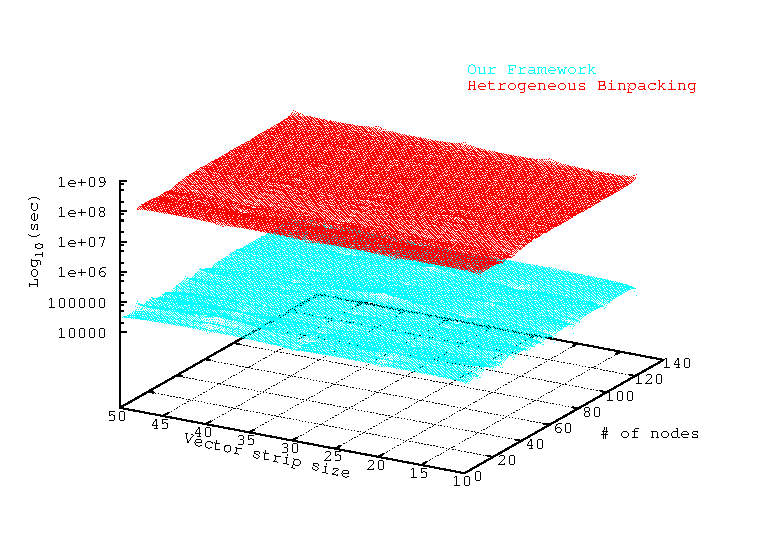
\includegraphics[angle=0, scale=0.33]{./figures/bin_surface}
    \label{fig:bin1ho}
  }
  \subfigure[2 Dimensional Convolution]{
    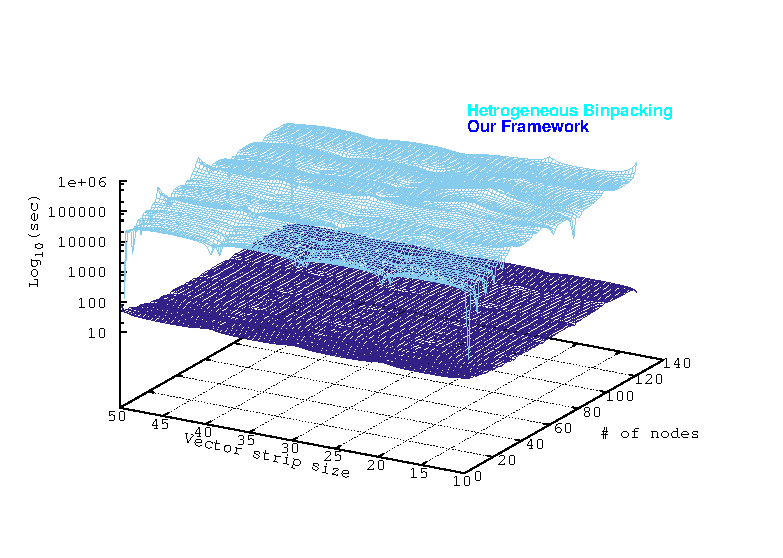
\includegraphics[angle=0, scale=0.33]{./figures/conv_surface}
    \label{fig:conv1ho}
  }
  \subfigure[Gram schmidtt linear-algebra kernel]{
    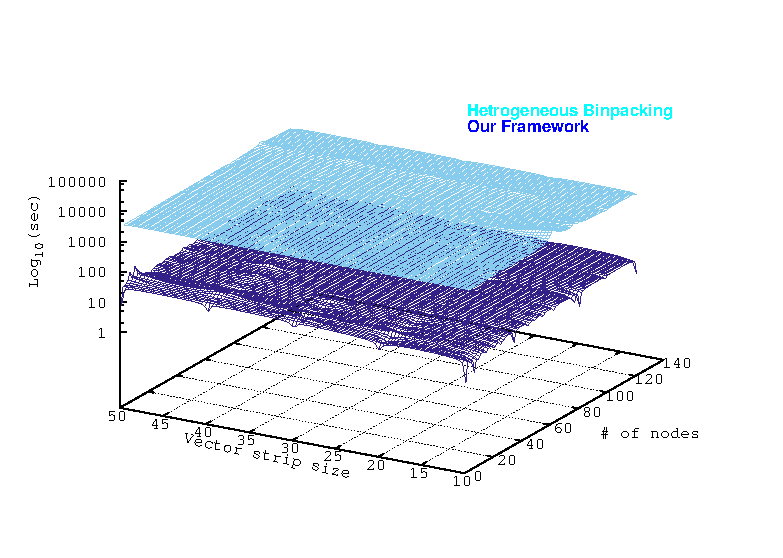
\includegraphics[angle=0, scale=0.33]{./figures/gram_surface}
    \label{fig:gram1ho}
  }
  \subfigure[2 Dimensional Seildel stencil computation]{
    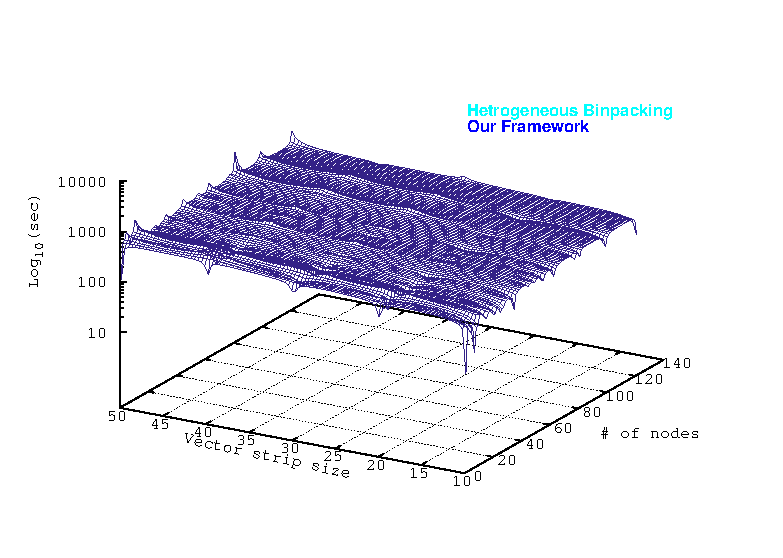
\includegraphics[angle=0, scale=0.33]{./figures/sei_surface}
    \label{fig:sei1ho}
  }
  \subfigure[2 Dimensional Jacobi stencil computation]{
    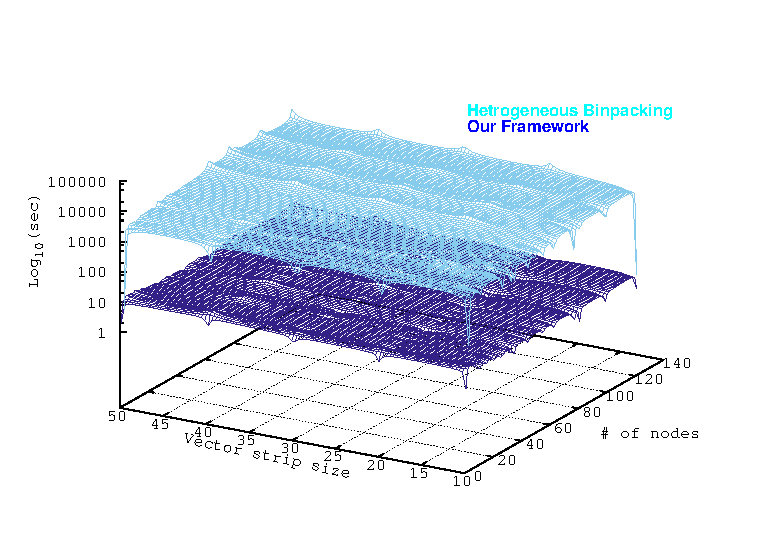
\includegraphics[angle=0, scale=0.33]{./figures/jac_surface}
    \label{fig:jacl1ho}
  }
  \caption{Comparison of execution times of ``Our Framework" and
    ``Heterogeneous Bin Packing"}
  \label{fig:ho}
\end{figure*}

\subsubsection{The results}
\label{sec:results-1}

The results for the experiments with the above experimental setup
comparing out approach with the aforementioned bin-packing approach is
shown in Figure~\ref{fig:ho}. Our approach performs better compared to
heterogeneous bin-packing for all the applications. The graphs in
Figure~\ref{fig:ho} consists of two surfaces layered on top of each
other. In these graphs the larger the value, the worse the latency (and
hence the performance of the application). For all graphs, the surface
representing the heterogeneous bin-packing solution is always layered
atop our results, which clearly show the superiority of our approach.

For seidel, the results for bin-packing could not be obtained, because the  
required
vector element length was larger than the available capability of the
underlying hardware. Our approach is able to deal with such a situation,
by fitting the required vector length to the capability and then running
the rest in an iterative manner.

NOTE: The experimental results section requires a lot more
refining. Basicaly a rewrite.

\subsection{More results}
\label{sec:more-results}

More results comparing the difference when the height of the dendrogram
is changed, etc.


%%% Local Variables: 
%%% mode: latex
%%% TeX-master: "bare_conf"
%%% End: 
